\documentclass[10pt]{beamer}
\usetheme{jambro}

\title[]{Macroeconomia I - Comportamento forward-looking e teoria do consumo}
\author[]{Paulo Victor da Fonseca}
\date{18 de abril de 2023}

\hypersetup{
    colorlinks = true,
    urlcolor = teal,
    linkcolor = teal    
}
\usepackage[portuguese]{babel}
\usepackage{subfig}
\usepackage{emoji}
\usepackage{hyperref}

\begin{document}

\begin{frame}[plain]
    \titlepage{
        \begin{center}
            \begin{minipage}{0.8\textwidth}
                \centering
            \end{minipage}
        \end{center}}
\end{frame}

\begin{frame}{Sumário}
    \tableofcontents
\end{frame}

\section{Comportamento forward-looking}
\begin{frame}
    {Comportamento forward-looking}
    \begin{itemize}
        \item Decisões de gastos no presente são influenciadas por \hlight{expectativas} com relação ao futuro\bigskip
        \item Portanto, há um componente \hlight{intertemporal} tanto para decisões de consumo quanto de investimento\bigskip
        \begin{enumerate}
            \item Famílias ajustam consumo corrente baseado em suas expectativas de renda futura: baixa renda corrente mas renda futura esperada elevada pode levar indivíduos a tomar empréstimos no presente, aumentar consumo e pagar dívidas no futuro - \textcolor{blue}{suavização do consumo}\medskip
            \item Decisões das firmas são baseadas em planos de negócios que incluem previsões de demanda futura pelos seus produtos e custos dos insumos. Investimento é intrinsicamente forward-looking dado que custos são incorridos no presente, mas fluxo de benefícios é realizado no futuro
        \end{enumerate}
    \end{itemize}
\end{frame}

\subsection{Valor presente}
\begin{frame}
    {Valor presente}
    \begin{itemize}
        \item O cálculo do \hlight{valor presente} de um fluxo de renda ou lucros futuros pode ser exemplificado pelas decisões de investimento\bigskip
        \item Uma firma maximizadora de lucros realizará projetos de investimento se retorno associado superar custos incorridos\bigskip
        \item Gastos com investimento, tipicamente, precedem retornos que podem ser irregulares e distribuídos ao longo do tempo\bigskip
        \item Lidamos com este fato calculando o \hlight{valor presente} ($V$) do fluxo esperado de lucros $\Pi$ ao longo do tempo
    \end{itemize}
\end{frame}

\begin{frame}
    {Valor presente}
    \begin{itemize}
        \item Com uma taxa de juros de 10\% a.a., se um indivíduo poupa \$100 hoje, receberá \$110 em um ano\bigskip
        \item De outra forma, \$110 no ano seguinte tem o mesmo valor que \$100 hoje, i.e., seu valor presente é \$100\bigskip
        \item De maneira geral, com uma taxa de juros constante e igual a $r$, o valor presente de $X$ unidades monetárias em $n$ anos é igual a $\frac{X}{(1 + r)^n}$ hoje\bigskip
        \item Portanto, o valor presente do fluxo esperado de lucros, $\Pi^e$, de um projeto de investimento com lucros ao longo de $T$ anos é dado por:
        \begin{equation}
            V_t^e = \Pi_t^e + \frac{\Pi_{t+1}^e}{(1 + r)} + \frac{\Pi_{t+2}^e}{(1 + r)^2} + \dots + \frac{\Pi_{t+T}^e}{(1 + r)^T} = \sum_{k = 0}^T \frac{1}{(1 + r)^k}\Pi_{t+k}^e\label{aula7_eq1}
        \end{equation}
    \end{itemize}
\end{frame}

\begin{frame}
    {Valor presente}
    \begin{itemize}
        \item Se custo de máquinas e equipamentos $>$ valor presente do fluxo de lucros, seria mais lucrativo colocar dinheiro no banco ou em títulos (que paguem taxa de juros $r$)\bigskip
        \item Se montante utilizado para aquisição de máquinas e equipamentos é obtido via empréstimos, se o custo superar o valor presente, esta aquisição não seria lucrativa\bigskip
        \item Por outro lado, se o valor presente $>$ custo, então, o investimento será lucrativo e uma firma maximizadora de lucros realizará o plano de investimento
    \end{itemize}
\end{frame}

\begin{frame}
    {Valor presente}
    \begin{itemize}
        \item Mesma lógica para modelar decisões de consumo\bigskip
        \item Futuro influencia decisões de consumo presente: calculamos valor presente do fluxo de renda esperado ao longo do período de vida do consumidor\bigskip
        \item Se assumirmos que indivíduo vive para sempre, o valor presente esperado de sua riqueza ao longo da vida, $\Psi^e$, em $t$ é dado por:
        \begin{equation}
            \Psi_t^e = (1 + r)A_{t-1} + \sum_{k=0}^\infty \frac{1}{(1 + r)^k}y_{t+k}^e\label{aula7_eq2}
        \end{equation}
        \begin{enumerate}
            \item $\sum_{k=0}^\infty \frac{1}{(1 + r)^k}y_{t+k}^e$: valor presente esperado dos rendimentos pós-taxação ao longo da vida\medskip
            \item $(1 + r)A_{t-1}$: recursos disponíveis em $t$ dos ativos mantidos ao final do período anterior
        \end{enumerate}
    \end{itemize}
\end{frame}

\section{Consumo}
\begin{frame}
    {Consumo}
    \begin{itemize}
        \item A renda de um indivíduo flutua ao longo do ciclo de vida\bigskip
        \item Também pode flutuar quando perde emprego, troca de posto de trabalho ou é promovido\bigskip
        \item Indivíduos preferem suavizar flutuações de seus rendimentos em suas decisões de consumo: devem levar em consideração expectativas futuras e ser capazes de tomar empréstimos ou poupar\bigskip
        \item Modelagens de decisões de consumo devem considerar como famílias formam expectativas com relação ao futuro e como poupam ou tomam empréstimos
    \end{itemize}
\end{frame}

\begin{frame}
    {Consumo}
    \begin{itemize}
        \item Desejo de suavizar consumo diante de flutuações de rendimentos é captado pela hipótese de utilidade marginal do consumo decrescente\bigskip
        \item Considere um modelo de 2 períodos\bigskip
        \item Se indivíduo sabe que renda será mais elevada no período seguinte, qual influência sobre decisão de consumo corrente?\bigskip
        \item Considere escolha entre: (i) baixo consumo ($=$ renda) no período 1 e consumo elevado ($=$ renda) no período 2; e (ii) a média dos dois níveis de consumo em cada um dos períodos\bigskip
        \item Se $U_{CC}(\bullet) < 0$, consumo maior sempre aumenta utilidade, mas aumentos sucessivos trazem benefícios cada vez menores\bigskip
        \item Portanto, famílias escolherão segunda opção: consumir média nos dois períodos oferece utilidade maior que primeira opção
    \end{itemize}
\end{frame}

\section{Hipótese da renda permanente}
\begin{frame}
    {Hipótese da renda permanente}
    \begin{itemize}
        \item A \hlight{hipótese da renda permanente} afirma que indivíduos escolhem, de maneira ótima, o quanto consumir de maneira a alocar seus recursos ao longo de seus ciclos de vida\bigskip
        \item Teoria desenvolvida, inicialmente, por Modigliani e Brumberg (1954)\bigskip
        \item Popularizada por Milton Friedman com o livro \emph{A theory of the consumption function} - 1957
    \end{itemize}
\end{frame}

\begin{frame}{Hipótese da renda permanente}
    \begin{figure}
        \centering
        \subfloat[\href{https://en.wikipedia.org/wiki/Franco_Modigliani}{Franco Modigliani (1918 - 2013)}\label{aula7_fig1}]{\href{https://en.wikipedia.org/wiki/Franco_Modigliani}{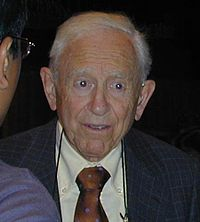
\includegraphics[width=0.3\textwidth]{./figures/aula7_fig1.jpg}}} \qquad
        \subfloat[\href{https://en.wikipedia.org/wiki/Milton_Friedman}{Milton Friedman (1912 - 2006)}\label{aula7_fig2}]{\href{https://en.wikipedia.org/wiki/Milton_Friedman}{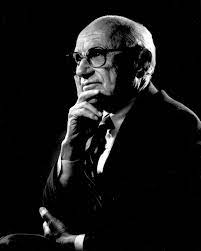
\includegraphics[width=0.27\textwidth]{./figures/aula7_fig2.jpeg}}}        
        %\caption{Bibliografia do curso}
        \label{aula7_fig1pih}
    \end{figure}
\end{frame}

\begin{frame}
    {Hipótese da renda permanente}
    \begin{itemize}
        \item Recursos de um indivíduo: ativos + renda presente e futura\bigskip
        \item A alocação de recursos ao longo do ciclo de vida é decisão \emph{forward-looking} e dependerá da taxa de juros, valor dos ativos e expectativas acerca de rendimentos e tributação futuros\bigskip
        \item Hipótese da renda permanente: trajetória de consumo ótima é suave quando comparada à da renda\bigskip
        \item E.g.: no início da vida laboral, rendimentos são baixos e, então, indivíduos tomam empréstimos para consumir mais\bigskip
        \item Quando renda aumenta, consumo é mantido constante e excedente de rendimentos é utilizado para pagar dívidas e poupar para aposentadoria\bigskip
        \item Na aposentadoria, rendimentos caem e, então, agentes retiram de suas poupanças
    \end{itemize}
\end{frame}

\begin{frame}
    {Hipótese da renda permanente}
    \begin{figure}
        \centering
        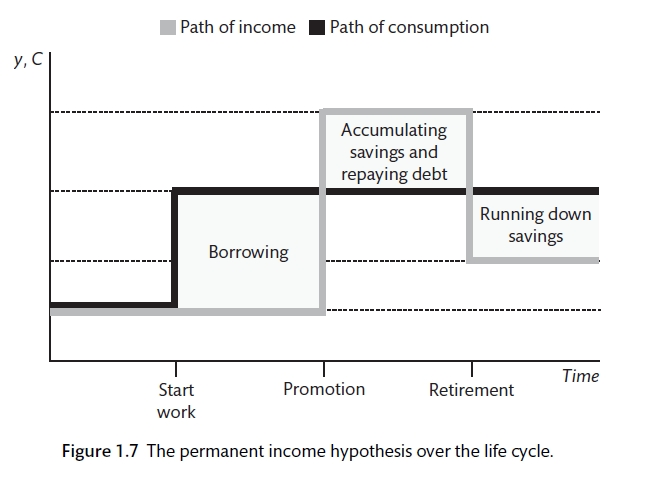
\includegraphics[width=0.6\textwidth]{./figures/aula7_fig3.jpg}
        \caption{Hipótese da renda permanente ao longo do ciclo de vida. Fonte: Carlin e Soskice (2015)}
    \end{figure}
\end{frame}

\begin{frame}
    {Hipótese da renda permanente}
    \begin{itemize}
        \item \hlight{Indivíduo irá contrair empréstimos e poupar para assegurar suavização da trajetória de consumo ao longo do ciclo de vida}\bigskip
        \item Analogamente, ao longo do ciclo de negócios, se indivíduo torna-se desempregado, contrai empréstimos para sustentar nível de consumo durante período de desemprego\bigskip
        \item A política fiscal tem papel relevante na suavizaçãod e consumo ao prover benefícios como seguro-desemprego (estabilizador automático)\bigskip
        \item HRP $\neq$ teoria de consumo Keynesiana (não há consideração explícita a respeito do futuro)
    \end{itemize}
\end{frame}

\begin{frame}
    {Hipótese da renda permanente}
    \begin{itemize}
        \item HRP: bom ponto inicial para pensarmos em escolha intertemporal e decisões de consumo \emph{forward-looking}\bigskip
        \item Como rendimentos oscilam ao longo do ciclo de vida, indivíduos contraem empréstimos/poupam para atingir objetivo de suavizar consumo\bigskip
        \item Mas é preferível uma trajetória de consumo constante em cada período, ou uma trajetória ascendente ou descendente de consumo?\bigskip
        \item Depende da relação entre taxa de juros sobre empréstimos e poupança e a taxa de trade-off entre consumo futuro e consumo presente do invidíduo\bigskip
        \item Esta última é a taxa de desconto subjetiva, $\rho$ - medida do grau de impaciência
    \end{itemize}
\end{frame}

\begin{frame}
    {Hipótese da renda permanente}
    \begin{itemize}
        \item Família escolhe trajetória de consumo que maximiza valor presente da utilidade (derivada do consumo) ao longo do ciclo de vida sujeito à restrição orçamentária intertemporal\bigskip
        \item Valor presente da utilidade intertemporal:
        \begin{equation}
            V_t^e = \sum_{k = 0}^\infty \frac{1}{(1 + \rho)^k}U(C_{t + k})
            \label{aula7_eq3}
        \end{equation}
        \item Utilidade de consumo descontada para período corrente pela taxa subjetiva de desconto intertemporal, $\rho$\bigskip
        \item Consumo futuro terá utilidade menor para consumidores mais impacientes\bigskip
        \item O valor presente esperado da riqueza total ao longo da vida é:
        \begin{equation}
            \Psi_t^e = (1 + r)A_{t-1} + \sum_{k=0}^\infty \frac{1}{(1 + r)^k}y_{t+k}^e
            \label{aula7_eq4} 
        \end{equation}
    \end{itemize}
\end{frame}

\begin{frame}
    {Hipótese da renda permanente}
    \begin{itemize}
        \item Restrição orçamentária pode ser escrita como:
        \begin{equation}
            A_t + C_t = (1 + r)A_{t-1} + y_t
            \label{aula7_eq5}
        \end{equation}
        \item Resolvendo problema de otimização dinâmica, obtemos a \hlight{equação de Euler}:
        \begin{equation}
            \tikz[tstyle]{\node[nstyle](node0){$U'(C_t)$}} = \tikz[tstyle]{\node[nstyle](node1){$\frac{1 + r}{1 + \rho}U'(C_{t+1}^e)$}}
            \label{aula7_eq6}
        \end{equation}
        \begin{tikzpicture}[tpstyle]
			\node[pencil,very thick, brick, draw, minimum height=0.8cm, minimum width=1.2cm] (box0) at (node0) {};
            \node[pencil,very thick,draw, minimum height=0.8cm, minimum width=2cm] (box1) at (node1) {};
		\end{tikzpicture}
        \item Eq. de Euler nos diz valor ótimo de $C_t$ em relação a $C_{t+1}^e$\bigskip
        \item No período corrente, indivíduo compara ganhos de consumir mais neste período com a perda descontada de consumir menos no período seguinte
        \begin{tikzpicture}[tpstyle]
			\draw[arrow, brick, ->] ([yshift=2pt]box0.west) to[bend left] +(-0.4,0.1) node[anchor=east,opacity=1] {\hand Ganho de consumir unidade adicional};
            \draw[arrow,->] ([yshift=2pt]box1.south west) to[bend right] +(+0.1,-0.3) node[anchor=west,opacity=1] {\hand VP subjetivo da perda de utilidade próx. período};
		\end{tikzpicture}
    \end{itemize}
\end{frame}

\begin{frame}
    {Hipótese da renda permanente}
    \begin{itemize}
        \item No próx. período, a renda do consumidor terá sido reduzida em uma magnitude $(1 + r)$, multiplicada pela utilidade marginal do consumo e pelo fator de impaciência\bigskip
        \item O consumidor não consegue atingir utilidade mais elevada do que quando o ganho de consumir uma unidade adicional no período corrente é exatamente equivalente ao valor presente subjetivo de perda de utilidade de consumir uma unidade adicional a menos no período seguinte
    \end{itemize}
\end{frame}

\begin{frame}
    {Hipótese da renda permanente}
    \begin{itemize}
        \item Eq. de Euler para utilidade logarítmica:
        \begin{eqnarray}
            \frac{1}{C_t} &=& \left(\frac{1 + r}{1 + \rho}\right) \frac{1}{C_{t+1}^e} \nonumber \\
            C_t &=& \left(\frac{1 + \rho}{1 + r}\right)C_{t+1}^e\label{aula7_eq7}
        \end{eqnarray}
        \item \hlight{Regra Keynes-Ramsey}: consumo crescente quando juro real $r$ maior que taxa de desconto $\rho$\bigskip        
        \item Se $r < \rho$, trajetória de consumo será decrescente
    \end{itemize}
\end{frame}

\begin{frame}
    {Hipótese da renda permanente}
    \begin{itemize}
        \item Intuição mais clara se $\rho = r$\bigskip
        \item Família obtem mesmo retorno (objetivo) ao poupar, $r$, que sua disposição (subjetiva) de trocar consumo presente por consumo futuro, $\rho$\bigskip
        \item Com $r = \rho$, \hlight{indivíduo prefere um nível constante de consumo em cada período do tempo}: $C_t = C_{t+1}^e$\bigskip
        \item O ponto crucial é que, independente de qual padrão de consumo seja prevalente, ele é independente das variações temporárias (período a período) de renda
    \end{itemize}
\end{frame}

\begin{frame}
    {Hipótese da renda permanente}
    \begin{itemize}
        \item Análises posteriores: assumiremos $\rho = r$\bigskip
        \item Para implementar plano ótimo de suavização do consumo ao longo do ciclo de vida, dada a renda de cada período, indivíduo deve poupar ou tomar empréstimo que for necessário para manter consumo constante\bigskip
        \item Se renda corrente está acima da renda permanente, indivíduo poupará\bigskip
        \item Caso contrário, toma emprestado
    \end{itemize}
\end{frame}

\begin{frame}
    {Hipótese da renda permanente}
    \begin{itemize}
        \item Se $\rho = r$, consumo em cada período é dado por:
        \begin{equation}
            C_t = \frac{r}{1 + r}\Psi_t^e\label{aula7_eq8}
        \end{equation}
        \item Intuição: consumidor poupa e toma empréstimo para obter trajetória de consumo perfeitamente suave (em expectativas)\bigskip
        \item A quantidade consumida em cada período é dada pelo valor de anuidade da riqueza esperada ao longo da vida: \hlight{renda permanente}\bigskip
        \item Indivíduo consome sua renda permanente e (\ref{aula7_eq8}) assegura que, em expectativa, o faz para sempre\bigskip
        \item Consumo permanece constante, a não ser que $\Psi_t^e$ se altere
    \end{itemize}
\end{frame}

\section{Predições e evidências empíricas}
\begin{frame}
    {Predições e evidências empíricas}
    \begin{itemize}
        \item Como consumo reage a variações na renda?\bigskip
        \begin{enumerate}
            \item \hlight{Mudanças antecipadas:} não devem impactar consumo dado que são incorporadas às decisões via ajustes no cálculo da renda permanente. \textcolor{purple}{Espera-se que a propensão marginal a consumir seja 0}. \underline{\textcolor{blue}{Excesso de sensibilidade} a variações antecipadas na renda contradizem o comportamento de} \newline \underline{suavização perfeita do consumo}\medskip
            \item \hlight{Mudanças não-antecipadas:} impactam consumo pois requerem ajustes no cálculo da riqueza futura ao longo da vida, $\Psi_t^e$ - variações não-antecipadas temporárias $\times$ permanentes
        \end{enumerate}
    \end{itemize}
\end{frame}

\begin{frame}
    {Predições e evidências empíricas}
    \begin{itemize}
        \item \textcolor{purple}{Mudança temporária e não antecipada.} Se a renda corrente, $y_t$, aumenta de maneira não-antecipada e temporária em uma unidade, o consumo aumenta na magnitude em que isto eleva a renda permanente\bigskip
        \item O aumento unitário será diluído ao longo do ciclo de vida\bigskip
        \item A função de consumo, então, nos diz que a renda permanente e, portanto, o consumo aumentarão apenas marginalmente: $r/(1 + r)$ vezes o aumento na renda permanente\bigskip
        \item Neste caso, a propensão marginal a consumir sobre uma renda transitória será de $r/(1+r)$\bigskip
        \item Se $r = 4\%$, $PMC = 3,8\%$
    \end{itemize}
\end{frame}

\begin{frame}
    {Predições e evidências empíricas}
    \begin{itemize}
        \item \textcolor{purple}{Mudança permanente e não antecipada.} Se $y_t$, aumenta em uma unidade para todos os valores de $t$, então, a renda permanente e consumo também aumentarão em uma unidade\bigskip
        \item A propensão marginal a consumir, dada a alíquota de impostos, sobre a renda permanente é igual a 1\bigskip
        \item Portanto, um \hlight{excesso de suavidade} do consumo em resposta a variações na renda permanente contradiz a hipótese de renda permanente neste caso
    \end{itemize}
\end{frame}

\begin{frame}{Excesso de sensibilidade a variações antecipadas na renda}
    \begin{tabular}{cl}
        \begin{tabular}{c}
            \href{https://www.nber.org/system/files/chapters/c10965/c10965.pdf}{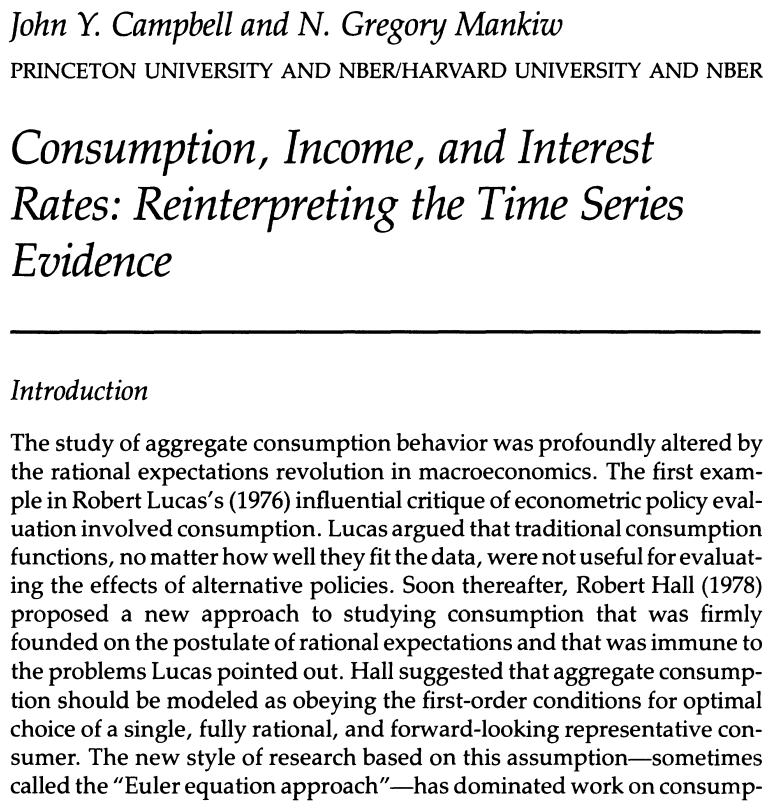
\includegraphics[width=3.5cm]{./figures/aula7_fig4.PNG}}            
        \end{tabular}
         & \begin{tabular}{l}
               \parbox{0.6\linewidth}{%  change the parbox width as appropiate
                   \begin{itemize}
                        \item A primeira hipótese testável sugere que não deve haver variações no consumo no momento do choque sobre a renda, caso a variação seja antecipada\medskip
                        \item \href{https://www.nber.org/system/files/chapters/c10965/c10965.pdf}{Campbell e Mankiw (1989)} testaram hipótese econometricamente com dados de consumo agregado e renda p/ países do G7\medskip
                        \item Estudo rejeita modelo no qual todos consumidores eram Ricardianos\medskip
                        \item Não pôde rejeitar modelo no qual 50\% eram Ricardianos e 50\% eram \emph{rule-of-thumb} (gastavam renda corrente)\medskip
                        \item Ou seja, consumo corrente era sensível a variações esperadas na renda para países do G7
                    \end{itemize}
               }
           \end{tabular} \\
    \end{tabular}
\end{frame}

\begin{frame}{Excesso de sensibilidade a variações antecipadas na renda}    
        \begin{figure}
            \centering
            \subfloat[\href{https://scholar.harvard.edu/campbell/home}{John Campbell}]{
\includegraphics[width=0.4\textwidth]{./figures/aula7_fig5.PNG}} \qquad
            \subfloat[\href{https://scholar.harvard.edu/mankiw/home}{Gregory Mankiw}]{
\includegraphics[width=0.4\textwidth]{./figures/aula7_fig6.PNG}}                        
        \end{figure}    
\end{frame}

\begin{frame}{Excesso de sensibilidade a variações antecipadas na renda}
    \begin{tabular}{cl}
        \begin{tabular}{c}
            \href{https://www.aeaweb.org/articles?id=10.1257/aer.96.5.1589}{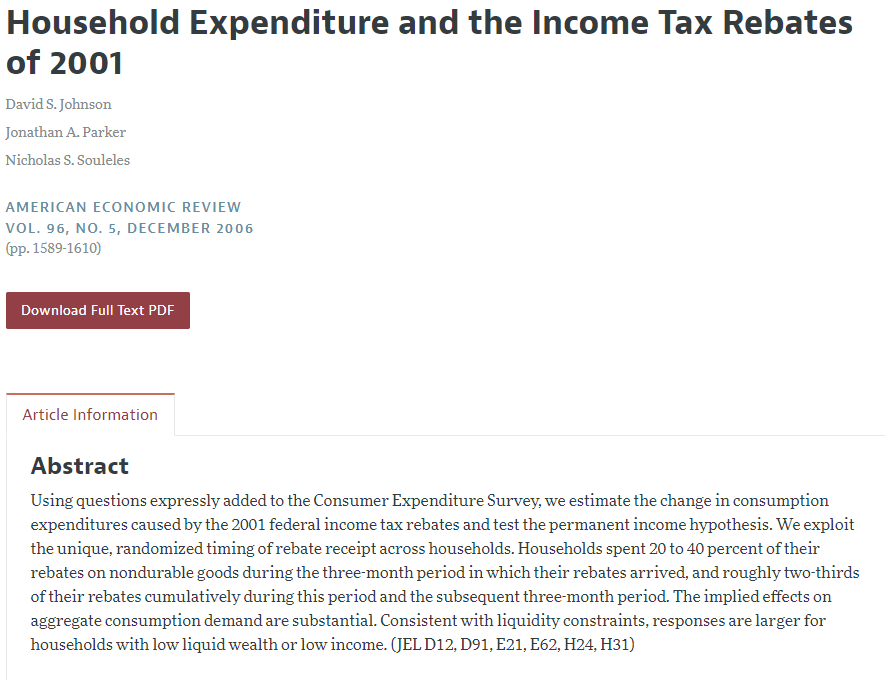
\includegraphics[width=3.5cm]{./figures/aula7_fig7.PNG}}            
        \end{tabular}
         & \begin{tabular}{l}
               \parbox{0.6\linewidth}{%  change the parbox width as appropiate
                   \begin{itemize}
                        \item De acorco com TRP, uma restituição de impostos temporária deve ter pequeno impacto sobre consumo e no momento do anúncio\medskip
                        \item \href{https://www.aeaweb.org/articles?id=10.1257/aer.96.5.1589}{Johnson, Parker e Souleles (2006)}, usando restituições de impostos federais nos EUA em 2001, identificaram o efeito causal de uma restituição de impostos\medskip
                        \item Consumidor médio gastava de 20 a 40\% da restituição (previsível) no período de 3 meses quando a restituição foi feita, ao invés de quando o programa foi anunciado\medskip
                        \item Famílias de baixa renda responderam de maneira mais forte - sugerindo relevância da restrição de crédito\medskip
                        \item Na literatura isso é conhecido como \hlight{excesso de sensibilidade} do consumo e é evidência contra fortes implicações do modelo de renda permanente
                    \end{itemize}
               }
           \end{tabular} \\
    \end{tabular}
\end{frame}

\begin{frame}{Excesso de sensibilidade a variações antecipadas na renda}    
    \begin{figure}
        \centering
        \subfloat[\href{https://micda.isr.umich.edu/people/david-s-johnson/}{David S. Johnson}]{
\includegraphics[width=0.3\textwidth]{./figures/aula7_fig8.jpg}} \qquad
        \subfloat[\href{https://mitsloan.mit.edu/faculty/directory/jonathan-a-parker}{Jonathan A. Parker}]{
\includegraphics[width=0.3\textwidth]{./figures/aula7_fig9.jpeg}} \qquad                       
        \subfloat[\href{https://fnce.wharton.upenn.edu/profile/souleles/}{Nicholas S. Souleles}]{
\includegraphics[width=0.3\textwidth]{./figures/aula7_fig10.jpg}}                        
    \end{figure}    
\end{frame}

\begin{frame}{Excesso de sensibilidade a variações antecipadas na renda}
    \begin{tabular}{cl}
        \begin{tabular}{c}
            \href{https://www.nber.org/system/files/working_papers/w15739/w15739.pdf}{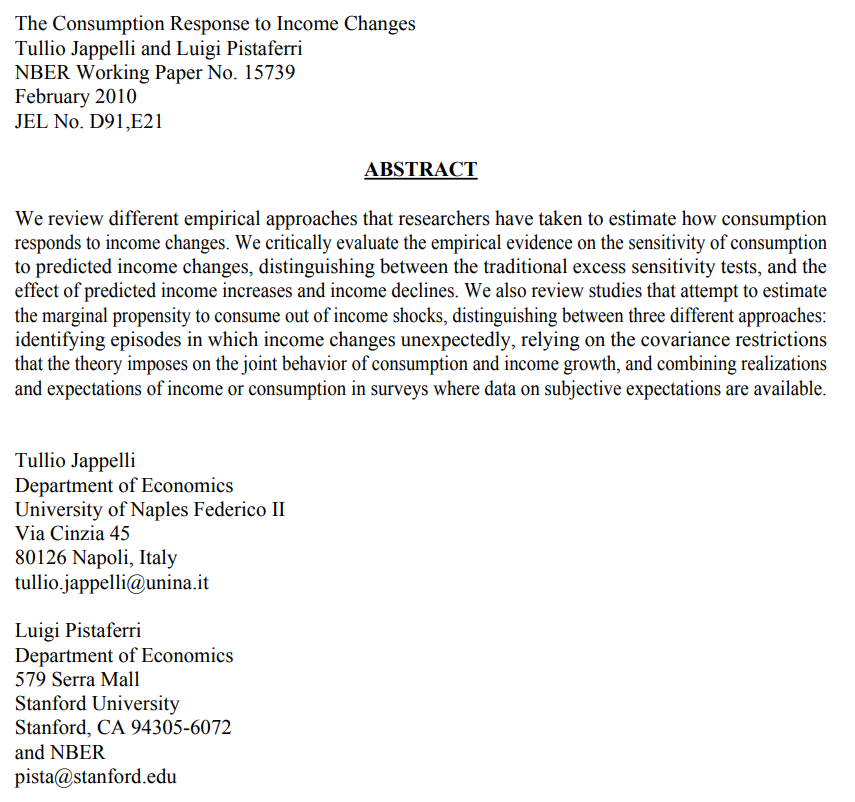
\includegraphics[width=3.5cm]{./figures/aula7_fig11.PNG}}            
        \end{tabular}
         & \begin{tabular}{l}
               \parbox{0.6\linewidth}{%  change the parbox width as appropiate
                   \begin{itemize}
                        \item Consumo é sensível a quedas previsíveis na renda devido à aposentadoria?\medskip
                        \item Evidência empírica sugere que sim\medskip
                        \item Apesar de violar HRP, existem explicações consistentes com suavização de consumo\medskip
                        \item Inclui a possibilidade de que consumo caia pois grande parte do consumo ao longo da vida está relacionado às atividades do trabalho\medskip
                        \item \href{https://www.nber.org/system/files/working_papers/w15739/w15739.pdf}{Jappelli e Pistaferri (2010)} concluem que as evidências do \emph{puzzle} consumo-aposentadoria não é uma contradição clara do princípio da renda permanente\medskip
                        \item Excesso de sensibilidade do consumo a aumentos antecipados na renda, mas não à queda, sugere importância da \hlight{restrição de crédito/liquidez}
                    \end{itemize}
               }
           \end{tabular} \\
    \end{tabular}
\end{frame}

\begin{frame}{Excesso de sensibilidade a variações antecipadas na renda}    
    \begin{figure}
        \centering
        \subfloat[\href{https://csef.it/people/tullio-jappelli/}{Tullio Jappelli}]{
\includegraphics[width=0.3\textwidth]{./figures/aula7_fig12.jpg}} \qquad
        \subfloat[\href{https://sites.google.com/view/pistaferri/home?authuser=0}{Luigi Pistaferri}]{
\includegraphics[width=0.3\textwidth]{./figures/aula7_fig13.PNG}}                        
    \end{figure}    
\end{frame}

\begin{frame}
    {Excesso de sensibilidade a variações na renda temporária e excesso de suavidade a variações na renda permanente}
    \begin{itemize}
        \item Estudos empíricos evidenciam que a resposta do consumo a choques de renda temporária é mais forte que previsto pela TRP\bigskip
        \item No caso de choques positivos de renda, isso viola predições da hipótese de renda permanente\bigskip
        \item Exemplo: forte resposta do consumo de veteranos norte-americanos da 2ª GM a pagamentos não-antecipados do \emph{National Service Life Insurance}\bigskip
        \item Esse tipo de evidência questiona hipótese de que consumidores tomam decisões otimizadoras levando em consideração horizontes temporais longos e possuem um baixo fator de desconto (igual à taxa de juros) para comparar consumo entre horizontes temporais distintos
    \end{itemize}
\end{frame}

\begin{frame}
    {Excesso de sensibilidade a variações na renda temporária e excesso de suavidade a variações na renda permanente}
    \begin{itemize}
        \item Consumidores respondendo a transferências não-antecipadas de renda aumentando nível de consumo sugere que taxa de desconto é maior do que assumida pela TRP: indivíduos são mais \hlight{impacientes}\bigskip
        \item Também é provável que a \hlight{incerteza} acerca da variação de renda observada (se temporária ou permanente) também pode fazer com que agentes não se comportem como previsto pela TRP\bigskip
        \item Se consumidor interpreta variação permanente de renda como temporária, então, consumiriam uma fração maior da variação da renda do que o consistente com o comportamento da TRP\bigskip
        \item Jappelli e Pistaferri (2010) revisaram evidências recentes e sugerem que, compatível com TRP, o consumo responde mais a variações na renda permanente do que na transitória\bigskip
        \item No entanto, não revisam suas decisões de consumo completamente quando há choques permanentes
    \end{itemize}
\end{frame}

\section{Restrição de crédito, impaciência e incerteza}
\begin{frame}
    {Restrição de crédito, impaciência e incerteza}
    \begin{itemize}
        \item Evidência empírica sugere que há 3 razões para que HRP não forneça um modelo adequado para consumo agregado:\bigskip
        \begin{enumerate}
            \item Presença de \hlight{restrições de crédito}, que impedem empréstimos de famílias que não possuem riqueza ou colateral\medskip
            \item \hlight{Impaciência}, impede que alguns consumidores consigam poupar como previsto pela HRP\medskip
            \item \hlight{Incerteza} acerca da trajetória de renda futura, que explica \textcolor{purple}{poupança precaucionária} acima do nível previsto pela HRP
        \end{enumerate}
    \end{itemize}
\end{frame}

\begin{frame}
    {Restrição de crédito}
    \begin{itemize}
        \item Se agentes preferem suavizar trajetória de consumo mas são impedidos pois não conseguem tomar empréstimos para manter consumo presente quando renda corrente está abaixo do nível de renda permanente, dizemos que são \textcolor{purple}{restritos por crédito}\bigskip
        \item Bancos se deparam com problemas informacionais para avaliar condições de crédito dos clientes e, então, nem sempre estão dispostos a disponibilizar crédito para consumidores cuja riqueza ou colateral seja insuficiente para assegurar empréstimo\bigskip        
    \end{itemize}
\end{frame}

\begin{frame}
    {Restrição de crédito}
    \begin{figure}
        \centering
        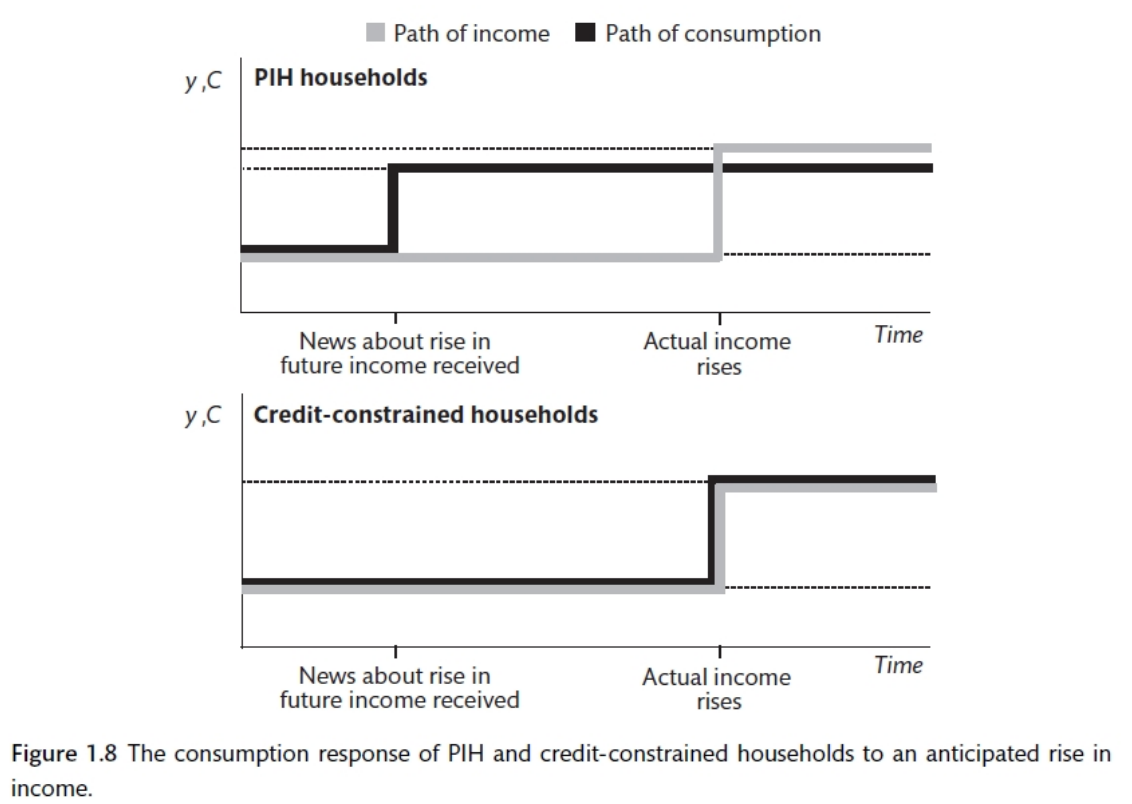
\includegraphics[width=0.6\textwidth]{./figures/aula7_fig14.PNG}
        \caption{Restrição de crédito e aumento antecipado de renda. Fonte: Carlin e Soskice (2015)}
    \end{figure}
\end{frame}

\begin{frame}
    {Restrição de crédito}
    \begin{itemize}
        \item A figura anterior mostra resposta de consumo de agentes Ricardianos e agentes com restrição de crédito frente a aumento antecipado de renda\bigskip
        \item Agentes Ricardianos contraem empréstimos para aumentar consumo assim que a notícia de renda mais alta chega\bigskip
        \item Consumidores com restrição de crédito não tem essa opção e, portanto, o consumo só aumenta quando a renda aumenta
    \end{itemize}
\end{frame}

\begin{frame}
    {Impaciência}
    \begin{itemize}
        \item A observação de que consumo de uma fração substancial dos consumidores varia um-pra-um com renda corrente (i.e., sem poupança ou empréstimo) reflete duas características\bigskip
        \item A mais importante é a presença de restrição de crédito\bigskip
        \item Que parece afetar, especialmente, consumidores mais jovens e de baixa renda\bigskip
        \item Restrição de crédito pode explicar a incapacidade dos agentes de contrair empréstimos para suavizar consumo\bigskip
        \item No entanto, não explica incapacidade de alguns agentes de poupar, o que permitiria suavização de consumo sem recorrer a empréstimos bancários
    \end{itemize}
\end{frame}

\begin{frame}
    {Restrição de crédito}
    \begin{figure}
        \centering
        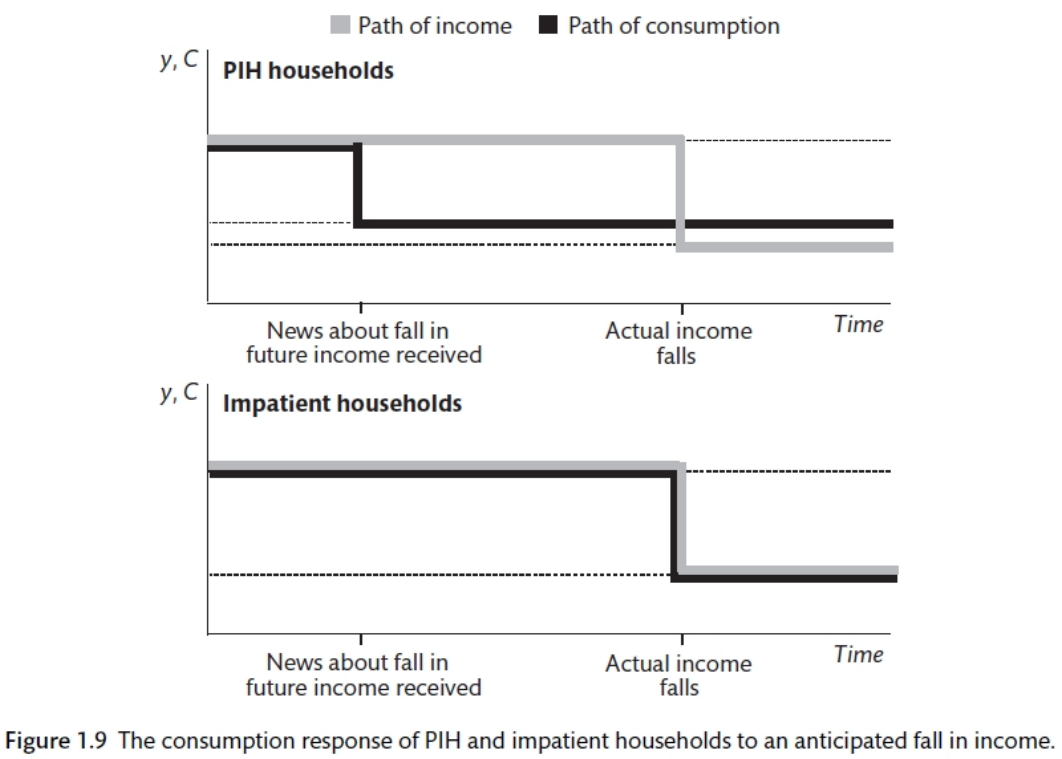
\includegraphics[width=0.6\textwidth]{./figures/aula7_fig15.PNG}
        \caption{Impaciência e quedas antecipadas de renda. Fonte: Carlin e Soskice (2015)}
    \end{figure}
\end{frame}

\begin{frame}
    {Impaciência}
    \begin{itemize}
        \item Parece existir não só consumidores com restrição de crédito mas, também, consumidores impacientes\bigskip
        \item Na figura anterior vemos a resposta de consumo para agentes Ricardianos e agentes impacientes a uma queda antecipada de renda\bigskip
        \item Agentes Ricardianos começam a poupar assim que recebem notícias de queda na renda futura, possibilitando suavização de consumo\bigskip
        \item Em contraste, agentes impacientes não conseguem reduzir consumo corrente assim que recebem notícias de queda na renda futura\bigskip
        \item Ou seja, o consumo corrente é reduzido drasticamente assim que a renda cai        
    \end{itemize}
\end{frame}

\begin{frame}
    {Impaciência: evidência experimental}
    \begin{itemize}
        \item Impaciência dos consumidores é representada por uma taxa de desconto mais elevada para o curto prazo que para o longo prazo\bigskip
        \item Considere a seguinte questão: se você estivesse decidindo hoje o que comer na semana seguinte, escolheria uma fruta ou chocolate?\bigskip
        \item Aproximadamente 3/4 dos entrevistados escolheriam fruta\bigskip
        \item No entanto, se questionados se comeriam fruta ou chocolate hoje, 70\% escolhe chocolate\bigskip
        \item Ou seja, preferências não são consistentes temporalmente
    \end{itemize}
\end{frame}

\begin{frame}
    {Impaciência: evidência experimental}
    \begin{itemize}
        \item Em um experimento, agentes possuem um orçamento e podem escolher entre 2 tipos de conta que pagam a mesma taxa de juros:\bigskip
        \begin{enumerate}
            \item Uma conta que não impõe restrições para saques\medskip
            \item Uma conta que impõe restrições para saques antes da data escolhida pelo participante\medskip
        \end{enumerate}
        \item Em uma visão puramente econômica, a conta irrestrita é preferível pois não impõe restrições sobre saques\bigskip
        \item Apesar disso, mais que metade dos investimentos é alocada na conta sob comprometimento\bigskip
        \item Isso revela desejo dos entrevistados para se comprometerem com a poupança
    \end{itemize}
\end{frame}

\begin{frame}
    {Impaciência: implicações para consumo e poupança}
    \begin{itemize}
        \item Diferenças consideráveis entre taxa de desconto no curto e longo prazo ajudam a explicar porque agentes, de forma simultânea, poupam em ativos ilíquidos como imóveis (baixa taxa de juros) e tomam empréstimos em cartões de créditos, pagando altas taxas de juros\bigskip
        \item Consumidores com este tipo de comportamento terão uma propensão marginal a consumir igual a 1\bigskip
        \item Mesmo que reconheçam que sua expectativa de bem estar seja mais elevada se pouparem mais hoje, podem ter dificuldade em resistir ao consumo e desviar do seu plano de poupança quando experienciam um aumento não-antecipado de renda\bigskip
        \item Uma forma de comprometimento a um plano de poupança é contrair uma hipoteca\bigskip
        \item Uma forma alternativa é o governo inscrever indivíduos em esquemas de poupança para aposentadorias, como pensões
    \end{itemize}
\end{frame}

\begin{frame}
    {Incerteza e poupança precaucionária}
    \begin{itemize}
        \item Se há incerteza acerca de oportunidades futuras de emprego ou saúde, então, agentes podem poupar como forma de se assegurar para contingências futuras\bigskip
        \item E.g., possuir um estoque de poupança pode ser importante para manter o nível de consumo no caso de perda de emprego por parte de um consumidor com restrição de crédito\bigskip
        \item Em situações de incerteza, consumidores tendem a poupar mais cedo que a HRP prediz\bigskip
        \item Ao invés de a propensão média a consumir decair à medida que a renda aumenta ao longo da vida (como na TRP), a poupança precaucionária leva a uma poupança antecipada fazendo com que o consumo aumente junto com a renda e, portanto, a propensão média a consumir aumenta mais tarde
    \end{itemize}
\end{frame}

\begin{frame}{\emoji{books} Bibliografia}
    \begin{itemize}
        \item BLANCHARD, O. Macroeconomia. 7.ed. São Paulo: Pearson Education do Brasil, 2017\medskip        
        \item CAMPBELL, J. Y.; MANKIW, N. G. (1989). Consumption, Income and Interest Rates: Reinterpreting the Time Series Evidence. In NBER Macroeconomics Annual 1989, Volume 4, NBER
        Chapters, pages 185–246. National Bureau of Economic Research, Inc.        
        \item CARLIN, W.; SOSKICE, D. Macroeconomics: Institutions, instability, and the financial system. Oxford, UK: Oxford University Press, 2015\medskip
        \item CHALLE, E. Macroeconomic fluctuations and policies. Cambridge, MA: The MIT Press, 2019.
        \item JAPPELLI, T.; PISTAFERRI, L. (2010). "The Consumption Response to Income Changes," Annual Review of Economics, Annual Reviews, vol. 2(1), pages 479-506, 09\medskip
        \item JOHNSON, D.S.; PARKER, J.A.; SOULELES, N.S. (2006). "Household Expenditure and the Income Tax Rebates of 2001," American Economic Review, American Economic Association, vol. 96(5), pages 1589-1610, December.
    \end{itemize}
\end{frame}
\end{document}